% =====================================================================
% Size-resolved confusion matrices, baseline vs recommended, both models.
% Generated by Confusion_original_improved/make_cm_figs.py from cm_values.json.
% =====================================================================
\begin{figure*}[t]
\centering
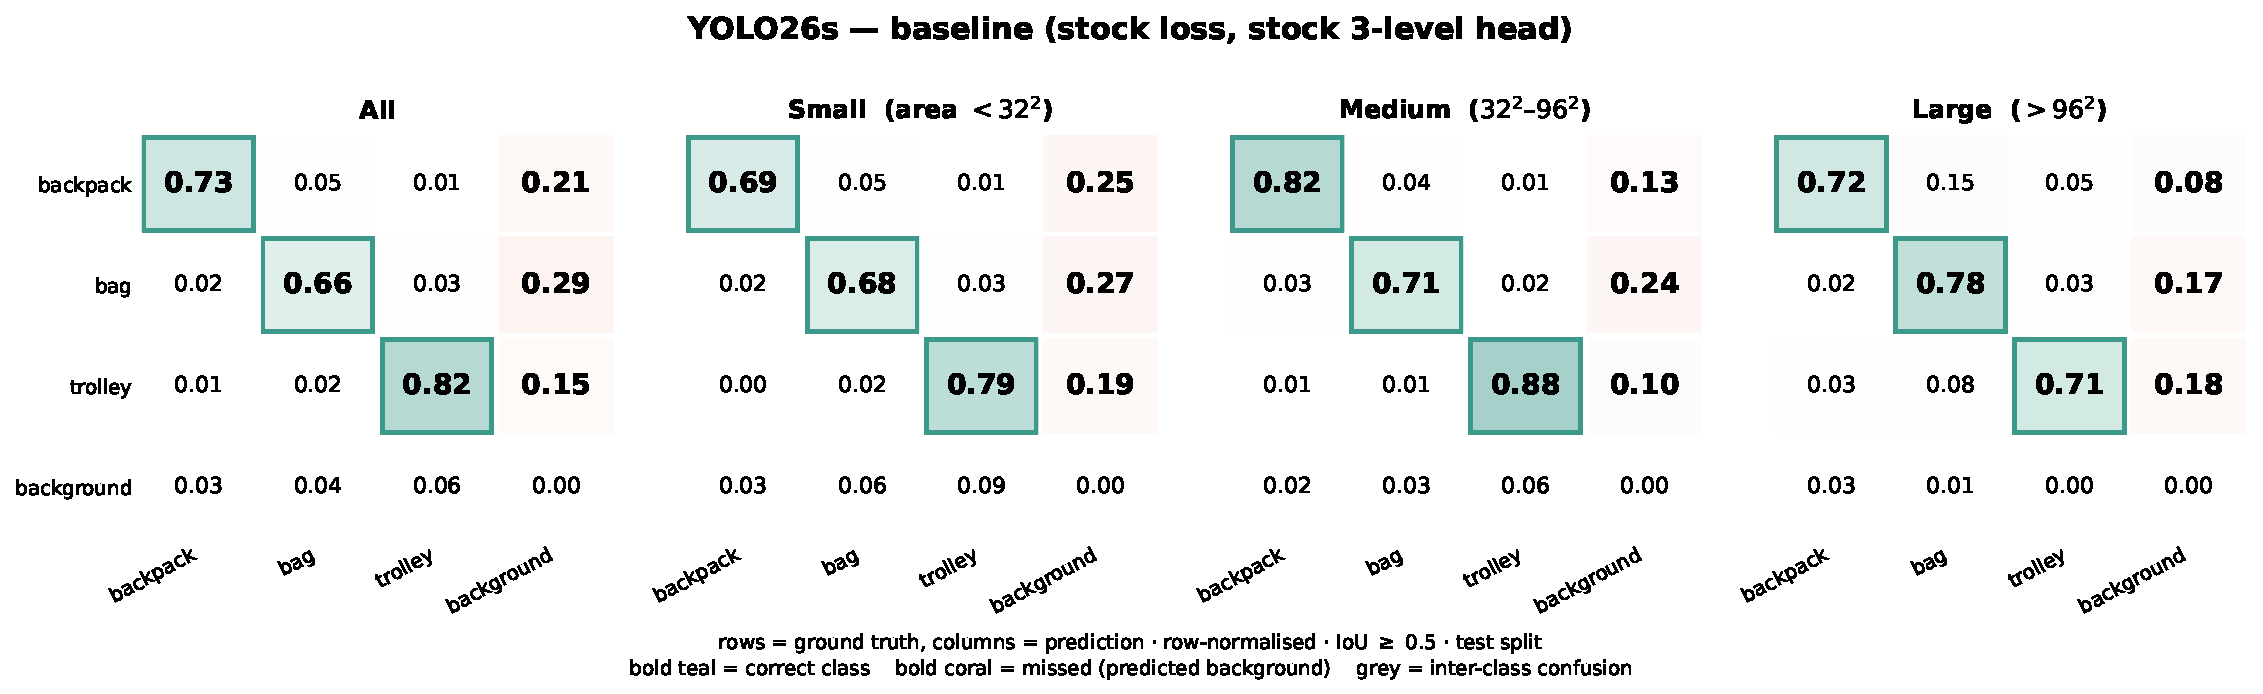
\includegraphics[width=\linewidth]{Confusion_original_improved/v26_default_cm.pdf}\\[5pt]
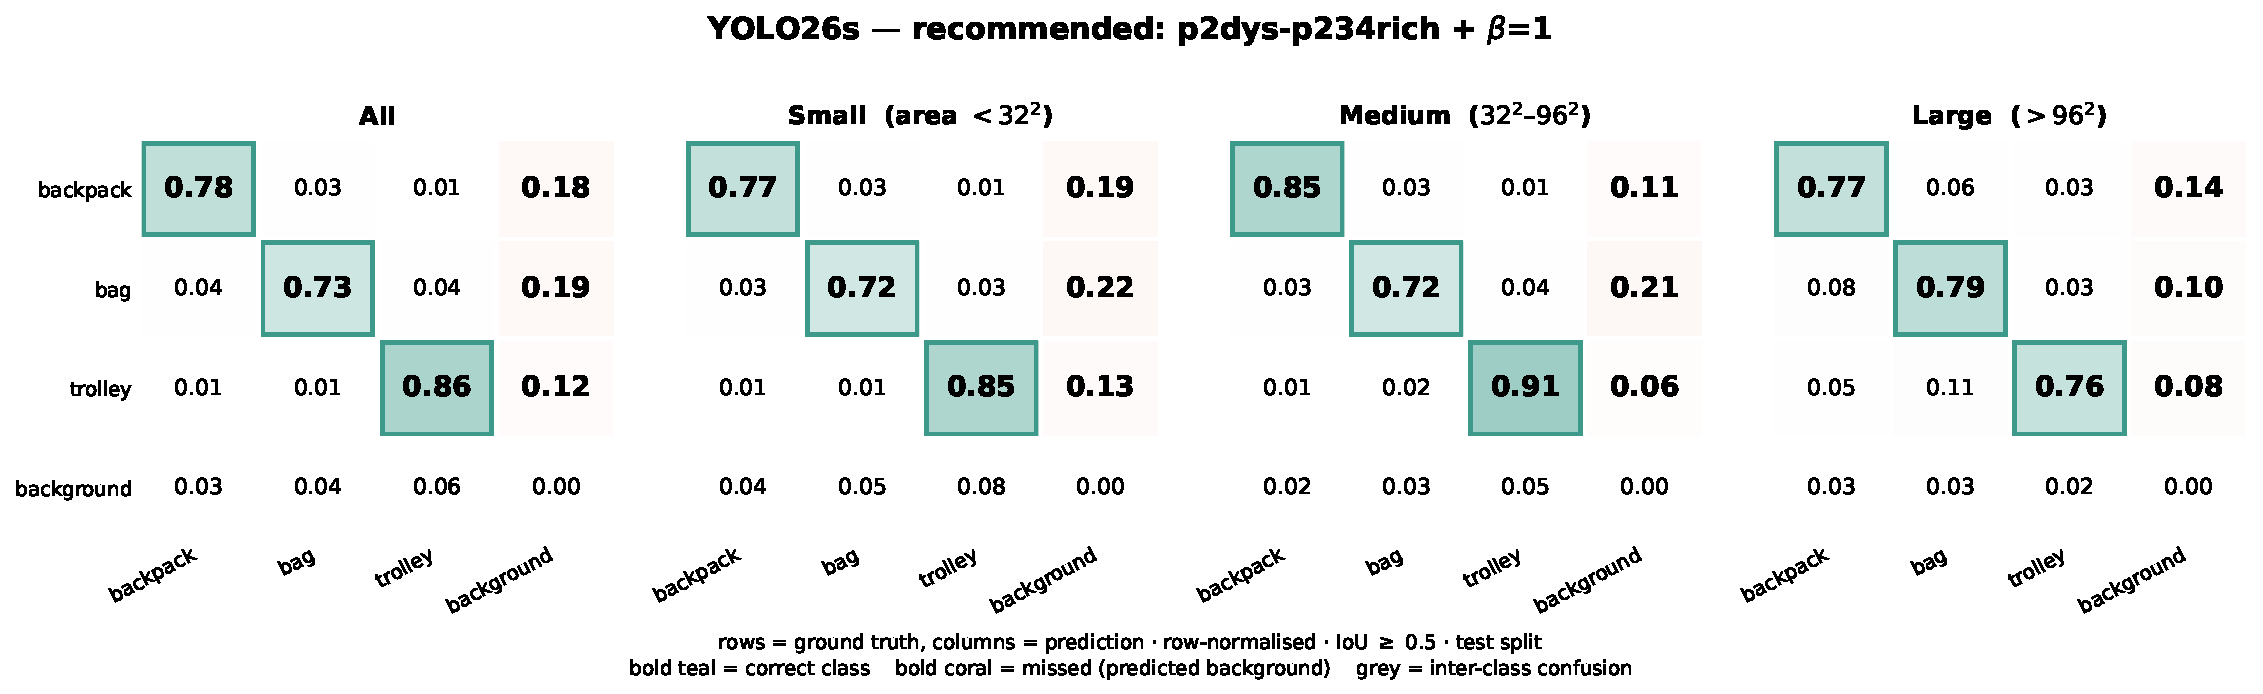
\includegraphics[width=\linewidth]{Confusion_original_improved/v26_custom_cm.pdf}
\caption{YOLO26s confusion, resolved by object size: baseline (top) and the
recommended configuration (bottom). Rows are ground truth, columns are
prediction, each row normalised, IoU $\geq 0.5$, test split. The bold teal
diagonal is the correct-class rate and the bold coral column is the \emph{miss}
rate --- ground truth predicted as background --- which for an alarm system is
the operative failure. Every class improves at every size; the largest single
change is \texttt{bag} missed to background, $0.29 \rightarrow 0.19$ overall and
$0.27 \rightarrow 0.22$ on small objects.}
\label{fig:cm26}
\end{figure*}

\begin{figure*}[t]
\centering
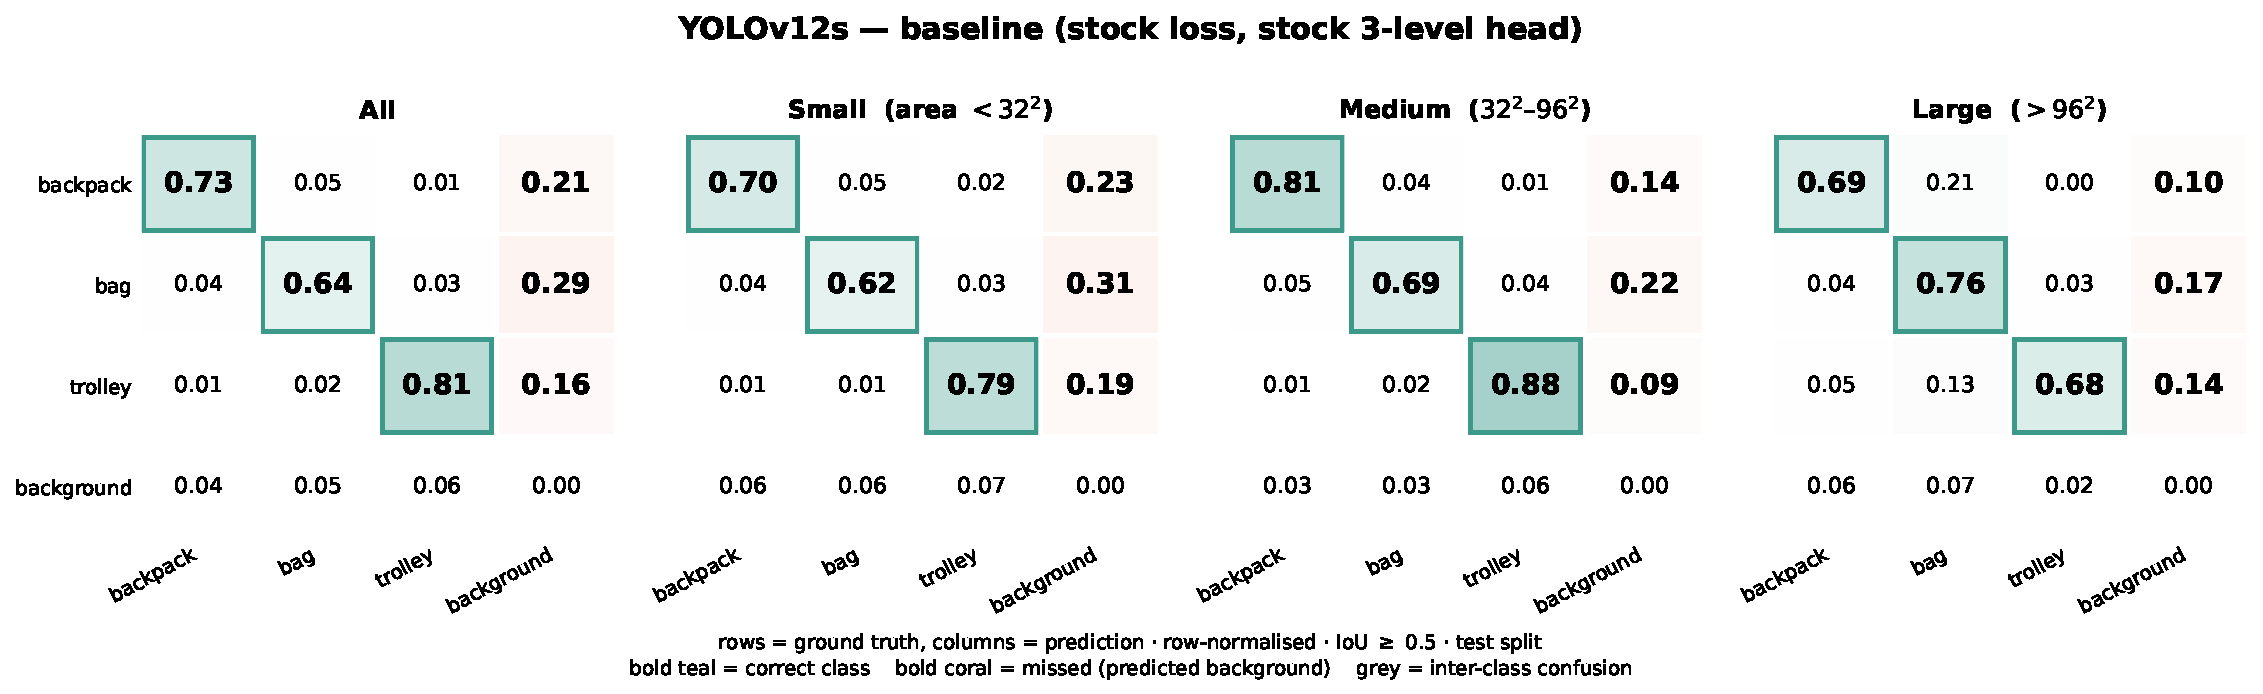
\includegraphics[width=\linewidth]{Confusion_original_improved/v12_default_cm.pdf}\\[5pt]
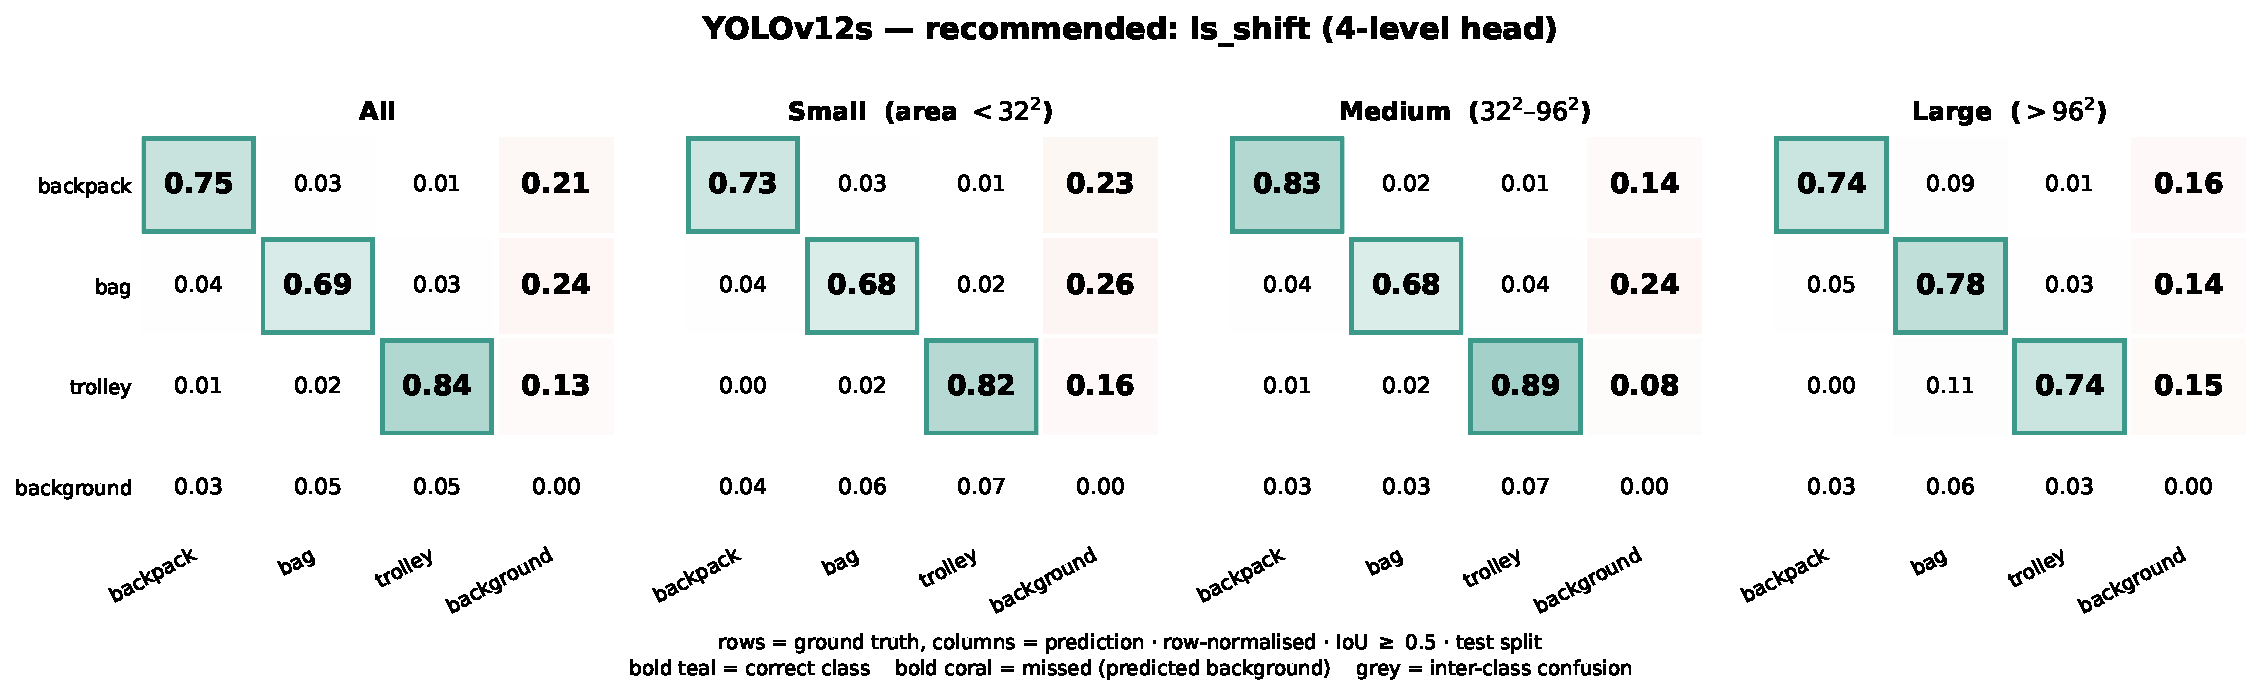
\includegraphics[width=\linewidth]{Confusion_original_improved/v12_custom_cm.pdf}
\caption{YOLOv12s confusion, same convention as Fig.~\ref{fig:cm26}: baseline
(top), recommended configuration (bottom). The pattern matches YOLO26 --- every
class improves at every size and \texttt{bag} improves most ($0.64 \rightarrow
0.69$ correct overall, misses $0.29 \rightarrow 0.24$) --- but from a lower
starting point on that class, and the residual \texttt{bag} miss rate stays
above YOLO26's.}
\label{fig:cm12}
\end{figure*}
